\section{Two-view Geometry}
Human see the world in binocular stereo vision, which allows them to have a good natural 3D understanding of the surrounding environments. Reproducing such multi-view image processing has the potential to enhance artificial vision algorithms, and has thus become a major challenge in computer vision.

The geometrical relationships between points visible in a two-view camera system can be represented in a matrix called the \emph{Essential Matrix} (when the intrinsic parameters of the cameras are known) or the \emph{Fundamental Matrix} (respectively when those parameters are unknown, which means that one has to compensate for it). In this chapter, we will focus on methods to estimate this matrix, and its use for aggregating geometrical information for stereo vision.

\subsection{Epipolar Geometry}
The basic setup of epipolar geometry is described in \autoref{fig:epipolar-geometry}.
\begin{figure}[H]
    \centering
    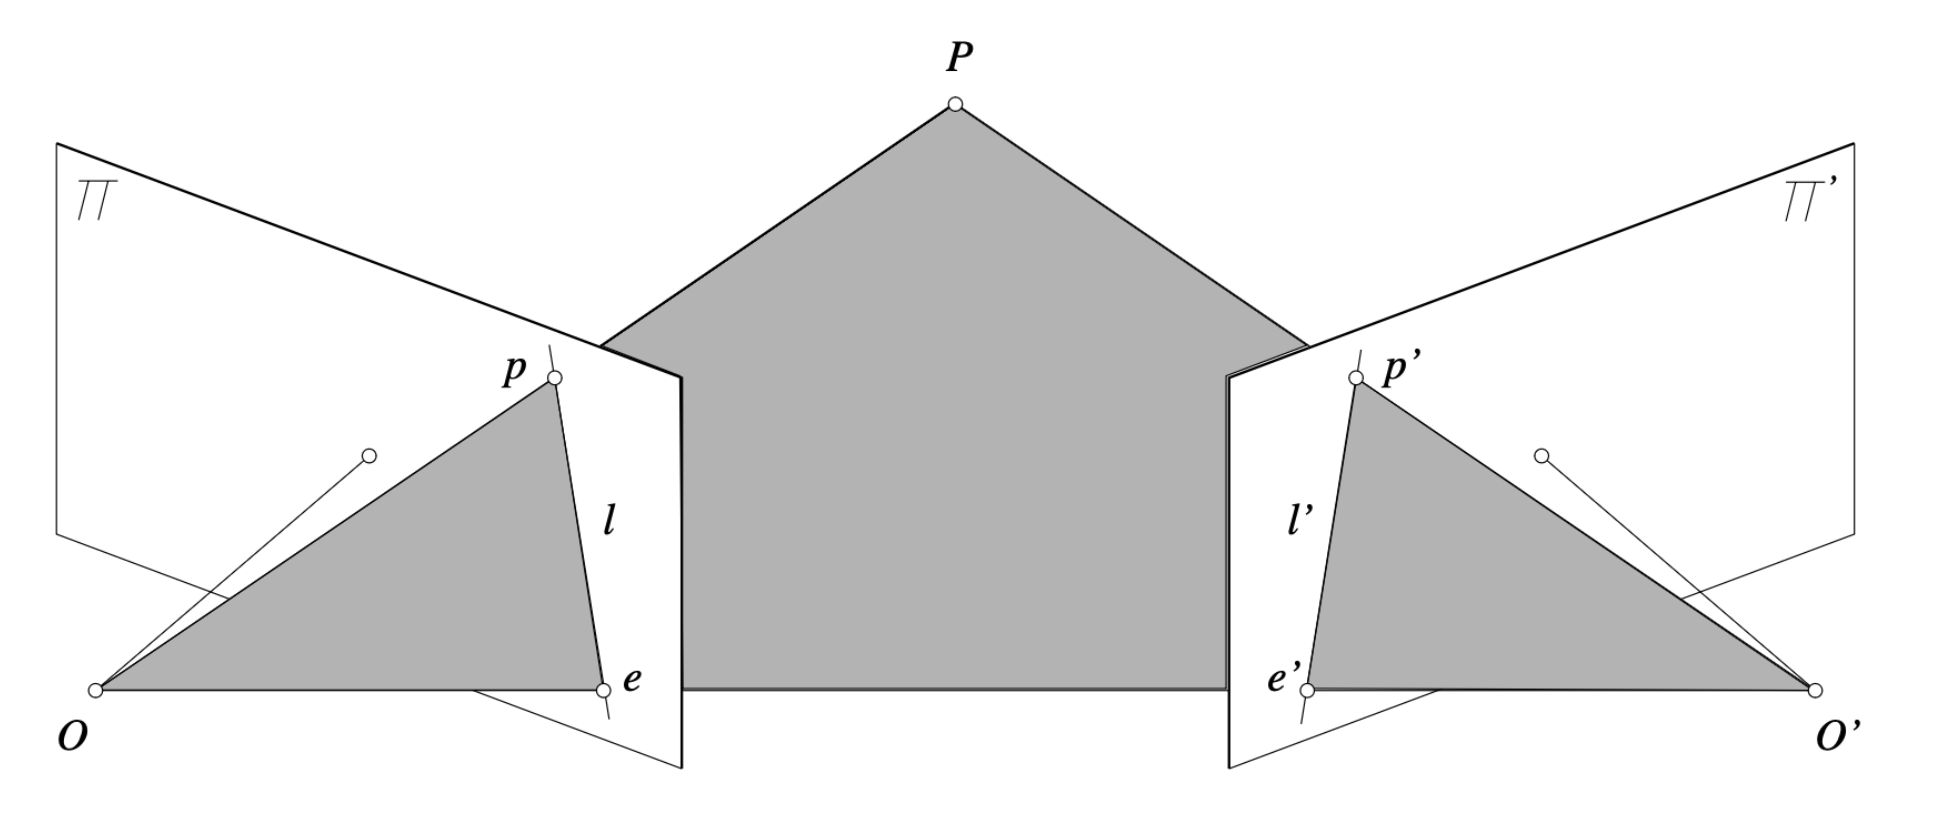
\includegraphics[width=.8\textwidth]{two-view/epipolar-geometry.png}
    \caption{Epipolar geometry.}
    \label{fig:epipolar-geometry}
\end{figure}
The scene is observed from two view points, caracterized by the two optical centers $O$ and $O'$, and their respective projected images (planes $\pi$ and $\pi'$). The line $OO'$ is called the \emph{baseline}, and cuts the planes respectively on $e$ and $e'$ called the \emph{epipoles}. 

The plane formed by $OPO'$ is called the \emph{epipolar plane}. Its intersection with $\pi$ is called the \emph{epipolar line} associated to $p'$, denote $l$. Respectively, its intersection with $\pi'$ is called the epipolar line associated to $p$ and is denoted $l'$.

\begin{remark}
    The epipolar line $l$ is associated with $p'$ and not $p$. This is due to the line $l$ being known whenever $p'$ is.
\end{remark}

\begin{theorem}[Epipolar constraint]
    \label{thm:epipolar-constraint}
    If a point $P$ is observed in two views in $p$ and $p'$, the observation $p$ \textbf{must belong} to the epipolar line associated to $p'$, namely $l$. Respectively, $p'$ must belong to the epipolar line $l'$ associated to $p$.
\end{theorem}

The epipolar constraint (Theorem \ref{thm:epipolar-constraint}) and the geometrical relationship between the two viewpoints' projections can be written as an equation, defining the \emph{Essential Matrix}, introduced by Longuet-Higgins and defined as follows (in the case of known intrinsic parameters):
\begin{equation}
    \label{eq:essential-matrix}
    p\cdot[t\times(\Rc p')]
\end{equation}
where $p=\begin{bmatrix}u\\v\\1\end{bmatrix}$ and $p'=\begin{bmatrix}u'\\v'\\1\end{bmatrix}$ denote the homogeneous coordinates of the observed points in the two view, $t$ is the coordinate vector of the translation $\overrightarrow{OO'}$ and $\Rc$ is the rotation matrix such that a free vector with coordinates $w'$ in the second coordinate system has coordinates $\Rc w'$ in the first coordinate system.

\autoref{eq:essential-matrix} can be rewritten as:
\begin{equation}
    p^\tp\Ec p' = 0
\end{equation}
where $\Ec=[t_\times]\Rc$.\footnote{For any vector $a$, $[a_\times]$ denotes the skew-symmetric matrix such that $[a_\times]b=a\times b$ is the cross-product of the vectors $a$ and $b$.} The matrix $\Ec$ is called the \emph{Essential Matrix}.

\begin{remark}
    Note that in practice, the expression of the essential matrix as $\Ec=[t_\times]\Rc$ does not matter, as we can directly estimate the matrix without computing the rotation and translation matrices. However, in the case of unknown intrinsic camera parameters, the full decomposition, and thus definition, would be different: one would have to compensate for the change of coordinate basis due to different camera parameters for the epipolar constraint to be verified. In this case, the fundamental matrix $F$ is defined such that:
    \begin{equation*}
        (Kp)^\tp F(K'p')=0
    \end{equation*}
    with $K$ and $K'$ the intrinsic parameters of the two cameras.
\end{remark}

\subsection{Essential matrix estimation}
We now assume that we are given a set of corresponding points from views $\pi$ and $\pi'$, with equal intrinsinc parameters, and denoted respectively as $p$ and $p'$. We know that such points must satisfy Theorem \ref{thm:epipolar-constraint}. Therefore, we can use this information to estimate the essential matrix $\Ec$, and use it to make correspondences between new points.

\begin{remark}
    In practice, Longuet-Higgins showed that at least 8 correspondences were needed to have a reasonable estimate of $\Ec$. In these notes, the algorithm is given for one single pair of points $(p,p')$, but it can be easily extended to multiple pairs $(p_i,p_i')_i$.
\end{remark}

Using \autoref{eq:essential-matrix}, we can write the epipolar constraint as:
\begin{equation}
    \begin{bmatrix}u&v&1\end{bmatrix}
    \begin{bmatrix}
        \Ec_{11} & \Ec_{12} & \Ec_{13} \\
        \Ec_{21} & \Ec_{22} & \Ec_{23} \\
        \Ec_{31} & \Ec_{32} & \Ec_{33}
    \end{bmatrix}
    \begin{bmatrix}u'\\v'\\1\end{bmatrix}=0
\end{equation}
which can be rewritten as:
\begin{equation*}
    \begin{bmatrix}
        uu' & uv' & u & vu' & vv' & v & u' & v' & 1
    \end{bmatrix}
    \begin{bmatrix}
        \Ec_{11} & \Ec_{12} & \Ec_{13} & \Ec_{21} & \Ec_{22} & \Ec_{23} & \Ec_{31} & \Ec_{32} & \Ec_{33}
    \end{bmatrix}^\tp=0
\end{equation*}

Similarly to camera calibration, instead of solving this ill-posed problem, Longuet-Higgins proposed to solve the linear least-squares problem:
\begin{equation}
    \label{eq:least-squares-essential}
    \argmin_{\norm{x}^2=1} \norm{Ax}^2
\end{equation}
where $A$ is the matrix of the $8$ correspondences, and $x$ is the vectorized form of $\Ec$. The solution to this approach is given by the singular value decomposition of $A$. Please refer to \autoref{subsec:least-squares-calibration} for more information.

\subsection{Epipolar lines}
In practice, trying to find $\Ec$ such that every point satisfied the epipolar constraint is equivalent to saying that $p$ should belong to the epipolar line associated to $p'$, and vice-versa. In practice, $p$ can be very close but will never exactly belong to the line, as the estimations introduce error. Thus, one might want to compute the average distance from the points to the epipolar lines associated to their respective corresponding points.

Once an estimate of $\Ec$ is obtained, the epipolar line associated to $p'$ is given by:
\begin{equation*}
    l = \Ec p'
\end{equation*}
The distance of a point $x=\begin{bmatrix}
    u\\v\\1
\end{bmatrix}$ to a line $l=\begin{bmatrix}
    a\\b\\c
\end{bmatrix}$ can be written as:
\begin{equation*}
    d(x,l) = \frac{|au+bv+c|}{\sqrt{a^2+b^2}}
\end{equation*}
This measure can give an idea of the quality of the estimate of $\Ec$. However, it is important to visualize the result, and it is necessary to draw the epipolar lines to have a better understanding of the quality of the estimate. For readability and interpretability, it is reasonable to draw segments instead of lines. They shall be centered in the projection of the associated point $p$ on the epipolar line $l$; we denote this projection $\hat{p}$.

Given a point $p=\begin{bmatrix}u\\v\\1\end{bmatrix}$, the projection of $p$ on the line $l=\begin{bmatrix}a\\b\\c\end{bmatrix}$ of direction $L:=\begin{bmatrix}a\\b\\0\end{bmatrix}$ is given by:
\begin{equation*}
    \hat{p} = p - p\cdot l\frac{L}{\norm{L}^2} = p-\frac{p\cdot l}{a^2+b^2}L = p-\frac{au+bv+c}{a^2+b^2}\begin{bmatrix}a\\b\\0\end{bmatrix}
\end{equation*}

Using these two formulae and basic linear algebra allow to recover the epipolar lines, to draw them, and to compute the distance with the points.

\subsection{Hartley's normalization}
The Longuet-Higgins approache described as \autoref{eq:least-squares-essential} is numerically poorly conditioned, and the estimations are often very inaccurate in practice. Hartley thus proposed an improvement of the algorithm, based on a rescaling of the data to ensure that the resulting matrix would satisfy the required properties of the essential or fundament matrix.

The idea is to center the data around 0, and to scale it such that the average distance to the origin is $\sqrt{2}$ (chosen empirically). This is done by applying the following transformation to the points $p$ and $p'$:
\begin{equation*}
    \begin{cases}
        \tilde{p} = Tp\\
        \tilde{p'} = T'p'
    \end{cases}
\end{equation*}
Such matrices $T$ and $T'$ can be computed by:
\begin{equation*}
    T = \begin{bmatrix}
        \sqrt{\frac{2}{\sigma^2}} & 0 & -\sqrt{\frac{2}{\sigma^2}}\mu_x \\
        0 & \sqrt{\frac{2}{\sigma^2}} & -\sqrt{\frac{2}{\sigma^2}}\mu_y \\
        0 & 0 & 1
    \end{bmatrix}
    \quad\text{and}\quad
    T' = \begin{bmatrix}
        \sqrt{\frac{2}{\sigma'^2}} & 0 & -\sqrt{\frac{2}{\sigma'^2}}\mu_x' \\
        0 & \sqrt{\frac{2}{\sigma'^2}} & -\sqrt{\frac{2}{\sigma'^2}}\mu_y' \\
        0 & 0 & 1
    \end{bmatrix}
\end{equation*}
where $\mu_x$ and $\mu_y$ are the average coordinate of $p$, and $\sigma$ is the average distance to the mean (average norm of the vector) for the point $p$.

We can now estimate the solution $\tilde{\Ec}$ by solving the least-squares problem associated with the constraint:
\begin{equation}
    \label{eq:normalized-essential}
    \tilde{p}^\tp\tilde{\Ec}\tilde{p'}=0
\end{equation}

The data having been normalized, it is necessary to impose a constraint on the estimated matrix $\tilde{\Ec}$ such that it respects the properties of the essential matrix: in particular, it should be of rank $2$. To enforce this rank-2 constraint, Hartley proposes to compute the SVD of $\tilde{\Ec}$, such that:
\begin{equation*}
    \tilde{\Ec} = U\Sigma V^\tp
\end{equation*}
where $\Sigma=\diag(r,s,t)$ with $r\leq s\leq t$ the singular values. Replacing $\Sigma$ by $\Sigma'=\diag(s,t,0)$, guarantees that the rank of the matrix is 2. We therefore define:
\begin{equation*}
    \tilde{\Ec}^* = U\Sigma^* V^\tp
\end{equation*}
which is a close estimate of $\tilde{\Ec}$ of rank 2.

From \autoref{eq:normalized-essential}, we can deduce that:
\begin{equation*}
    (Tp)^\tp\tilde{\Ec}^*(T'p')\simeq0
\end{equation*}
and thus, we can recover the final estimate of the essential matrix by projecting back the normalized data to the original coordinate basis:
\begin{equation*}
    \Ec = T\tilde{\Ec}^*T'
\end{equation*}

In practice, the estimate using Hartley's normalization improves the results by a significant margin, especially for a small number of points (such as 8).